% !TeX root = ../seminar.tex
% Backup slides: not counted in the frame numbers (appendixnumberbeamer).
\section*{Backup}

\begin{frame}[plain]
\vfill
\centering
{\usebeamerfont{title}\usebeamercolor[fg]{title}\Large Backup slides}
\vfill
\end{frame}

\begin{frame}{Backup: what goes into a mass forecast?}
For small, jointly estimated uncertainties, propagate the covariance in the two fitted scales:
\[
 \sigma^2(\ln \Ml)=\sigma^2(\ln\tetE)+\sigma^2(\ln\piE)
       -2\,\mathrm{cov}(\ln\tetE,\ln\piE).
\]
\begin{itemize}
  \item The first overview forecast used separate photometric and astrometric Fisher blocks,
        with the mass error calculated from fractional errors in quadrature.
  \item In a real fit, the baseline includes source position, proper motion and source parallax.
        Neighbouring light can shift the reference centroid as the source brightens.
  \item Fisher errors describe the local curvature near the simulated parameters.
        Sparse coverage can leave disconnected solutions that require fits to explore.
\end{itemize}
\refnote{First overview report, sections on mass inference and Fisher forecasts.}
\note{In the full model, for an angular source radius $\theta_\star$ inferred independently, a detectable
      finite-source signature can also constrain $\rho=\theta_\star/\tetE$ and hence $\tetE$.
      The September headline analysis used a point source.}
\end{frame}

\begin{frame}{Backup: a compact-object precision cross-check}
\centering
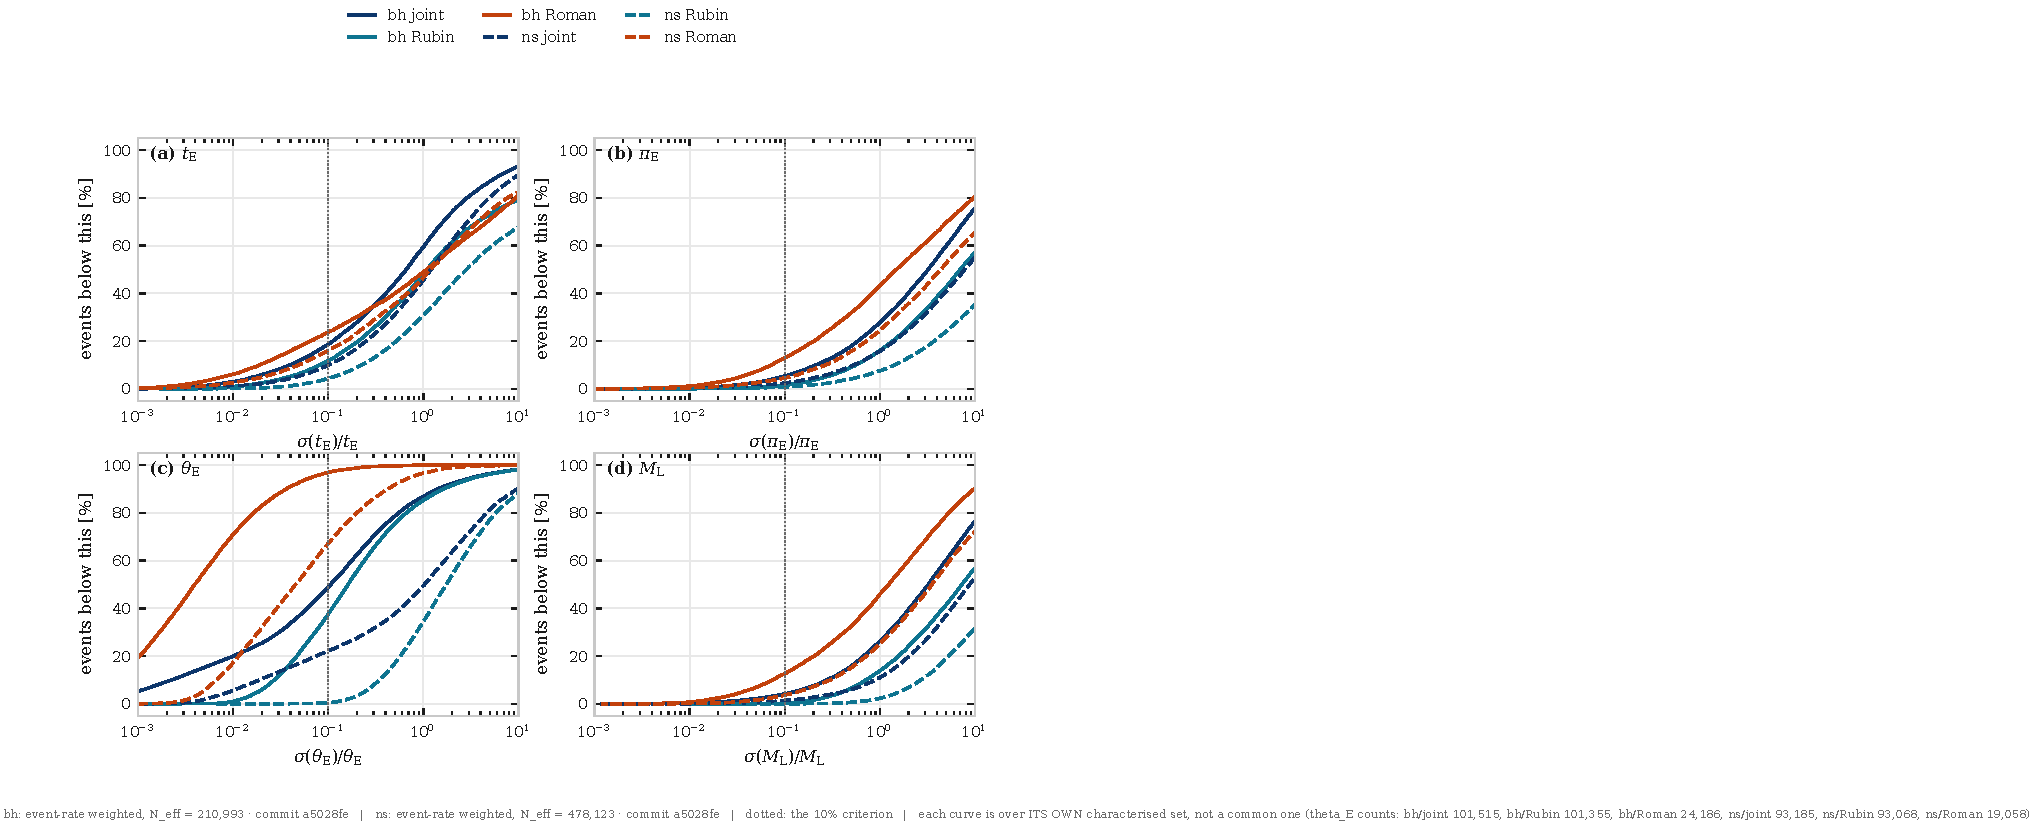
\includegraphics[height=.60\paperheight, trim=0 14 508 0, clip]{p7_precision}\\[2pt]
\refnote{September simulations. Event-rate-weighted cumulative fractional errors. Each curve uses
its own survey and parameter sample. Compare precision gains on a common set of events.}
\note{For the Roman black-hole forecasts the effective sample size is about $8{,}700$. The
      effective sample sizes printed inside the original plot refer to all draws in each population,
      so they should not be used as the sample size of a selected curve.}
\end{frame}

\begin{frame}{Backup: the astrometric signal scale}
\vspace{1mm}
\begin{columns}[c]
\begin{column}{.56\linewidth}
\centering
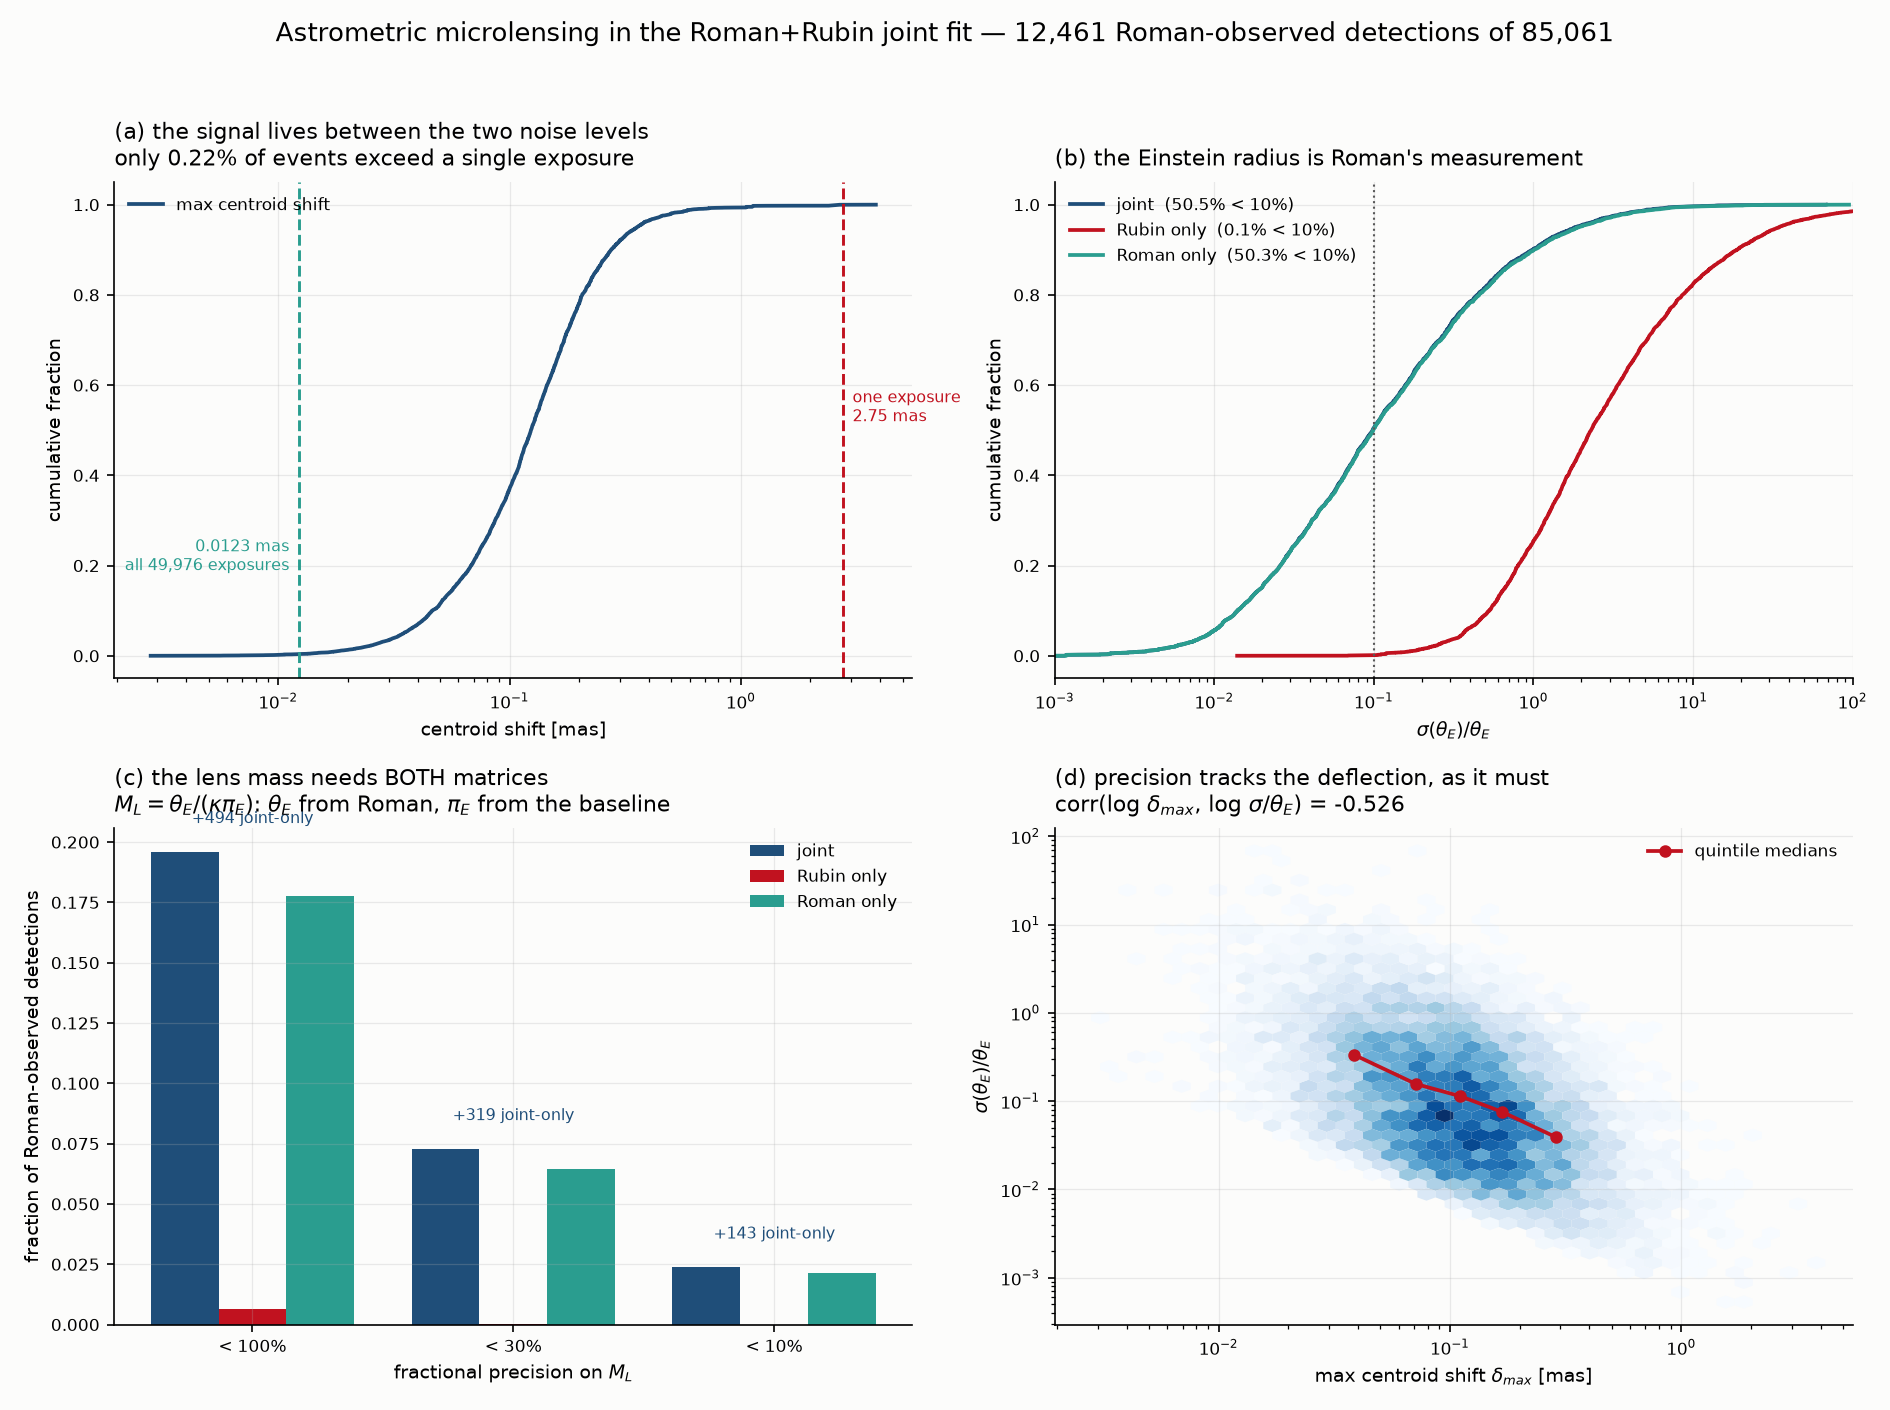
\includegraphics[width=.94\linewidth]{h5_astrometry_summary}\\[1mm]
\refnote{Ordinary lenses in Roman's fields, as simulated.}
\end{column}
\begin{column}{.40\linewidth}
\begin{itemize}\setlength{\itemsep}{6pt}
  \item \textbf{Black holes}: $3.4$\,mas median maximum shift in Roman detections
  \item \textbf{Ordinary lenses}: $0.12$\,mas; the forecast relies on repeated exposures
  \item Rubin adds little to Roman's typical $\tetE$ forecast
\end{itemize}
\vspace{4mm}
{%
\begin{beamercolorbox}[rounded=true,sep=5pt,wd=\linewidth]{block body alerted}
\centering Risk: does the $1.1$\,mas floor average down?
\end{beamercolorbox}}
\end{column}
\end{columns}
\vfill
\refnote{Astrometric floor: \ads{2019JATIS...5d4005S}{Sanderson et al.\ 2019}}
\note{\begin{itemize}
  \item The $1.1$\,mas bright-source floor in the first overview is a model input. Actual visit errors
        depend on source brightness, and high-cadence visits need not be independent.
  \item The listed medians are after the dust adjustment. Their underlying Roman detection samples had
        $\Neff$ of about $8{,}600$ (black holes) and $3{,}700$ (ordinary lenses) before the adjustment.
  \item An event's maximum centroid shift and the error on its fitted Einstein radius are different
        quantities. Joint time coverage and modelling the unlensed track also matter.
\end{itemize}}
\end{frame}

\begin{frame}{Backup: seeing the two images}
\vspace{1mm}
\begin{columns}[c]
\begin{column}{.56\linewidth}
\centering
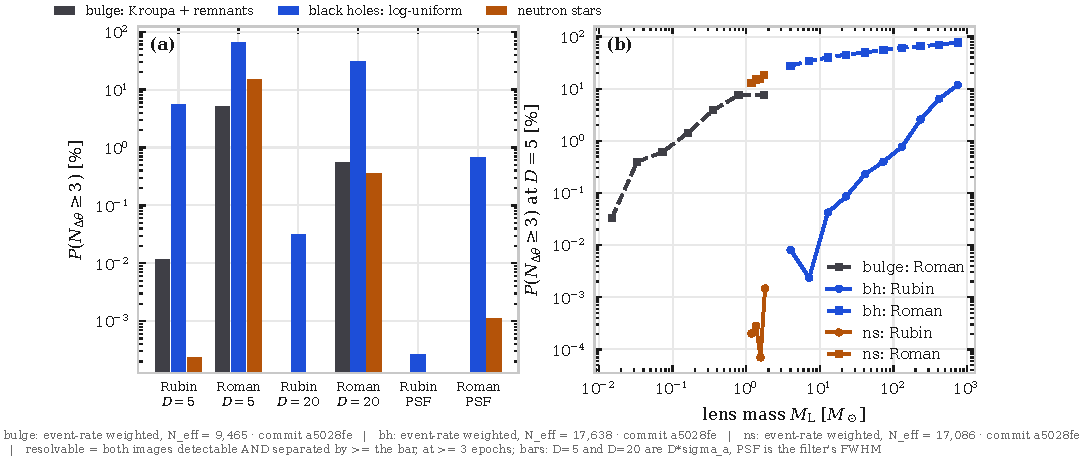
\includegraphics[width=.94\linewidth]{p6_resolution}\\[1mm]
\refnote{(a) by population, telescope and criterion; (b) against lens mass. Figure as simulated.}
\end{column}
\begin{column}{.40\linewidth}
\[
  \Delta\theta = \tetE\sqrt{u^2+4}
\]
{Roman black-hole detections,\\ dust-adjusted:\\[3pt]
\begin{tabular}{@{}ll@{}}
generous bar & $34\%$ \\
strict bar & $15\%$ \\
PSF width & $0.25\%$
\end{tabular}}
\vspace{5mm}

{%
\begin{beamercolorbox}[rounded=true,sep=5pt,wd=\linewidth]{block body alerted}
\centering Simulated Roman images can test which thresholds are realistic.
\end{beamercolorbox}}
\end{column}
\end{columns}
\vfill
\refnote{Criterion: \ads{2026ApJ..1009..116S}{Sajadian \& Makler 2026, ApJ 1009, 116}}
\note{\begin{itemize}
  \item Resolvable: at least three visits with both images detectable and $\Delta\theta$ above a bar:
        $\mathcal{D}\sigma_{\rm ast}$ with $\mathcal{D}=5$ (generous) or $20$ (strict), or the PSF width.
  \item Rubin resolves $\approx5\%$ of its black-hole events at the generous bar; for lighter lenses resolution is rare.
  \item The predicted fractions span two orders of magnitude. The criterion for Roman's diffraction-limited images must be
        measured on simulated Roman images.
\end{itemize}}
\end{frame}

\begin{frame}{Backup: a central transit of an extended star}
\centering
\vspace{2mm}
\animategraphics[autoplay, loop, controls=off, poster=31, width=.76\linewidth]{16}{img/anim/frame_}{00}{80}

\vspace{4mm}
A ring appears at exact centre alignment in this example.\\ Most events pass well outside the source disc.
\vfill
\refnote{Reverse ray tracing of a limb-darkened star, $\theta_\star=0.6\,\tetE$ (A.~Salehi); the curves are
measured from the traced images.}
\note{\begin{itemize}
  \item In a real event the images are too close to separate: a telescope sees only their total light and its centre.
  \item At exact centre alignment the ring is symmetric. During the transit the finite source caps the
        magnification and reverses the centroid shift. Dashed grey: a point source.
\end{itemize}}
\end{frame}

\begin{frame}{Backup: light curves and centroid shifts for several $u_0$}
\centering
\vspace{2mm}
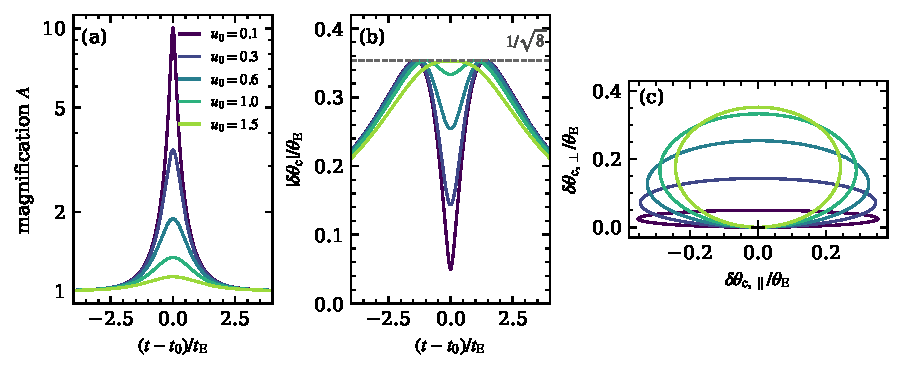
\includegraphics[width=.86\linewidth]{theory_curves}\\[3mm]

\small (a) magnification, (b) centroid shift against time, (c) the centroid's ellipse on the sky.
\end{frame}

\begin{frame}{Backup: gap filling --- when Rubin matters inside Roman's fields}
\begin{columns}[T]
\begin{column}{.56\linewidth}
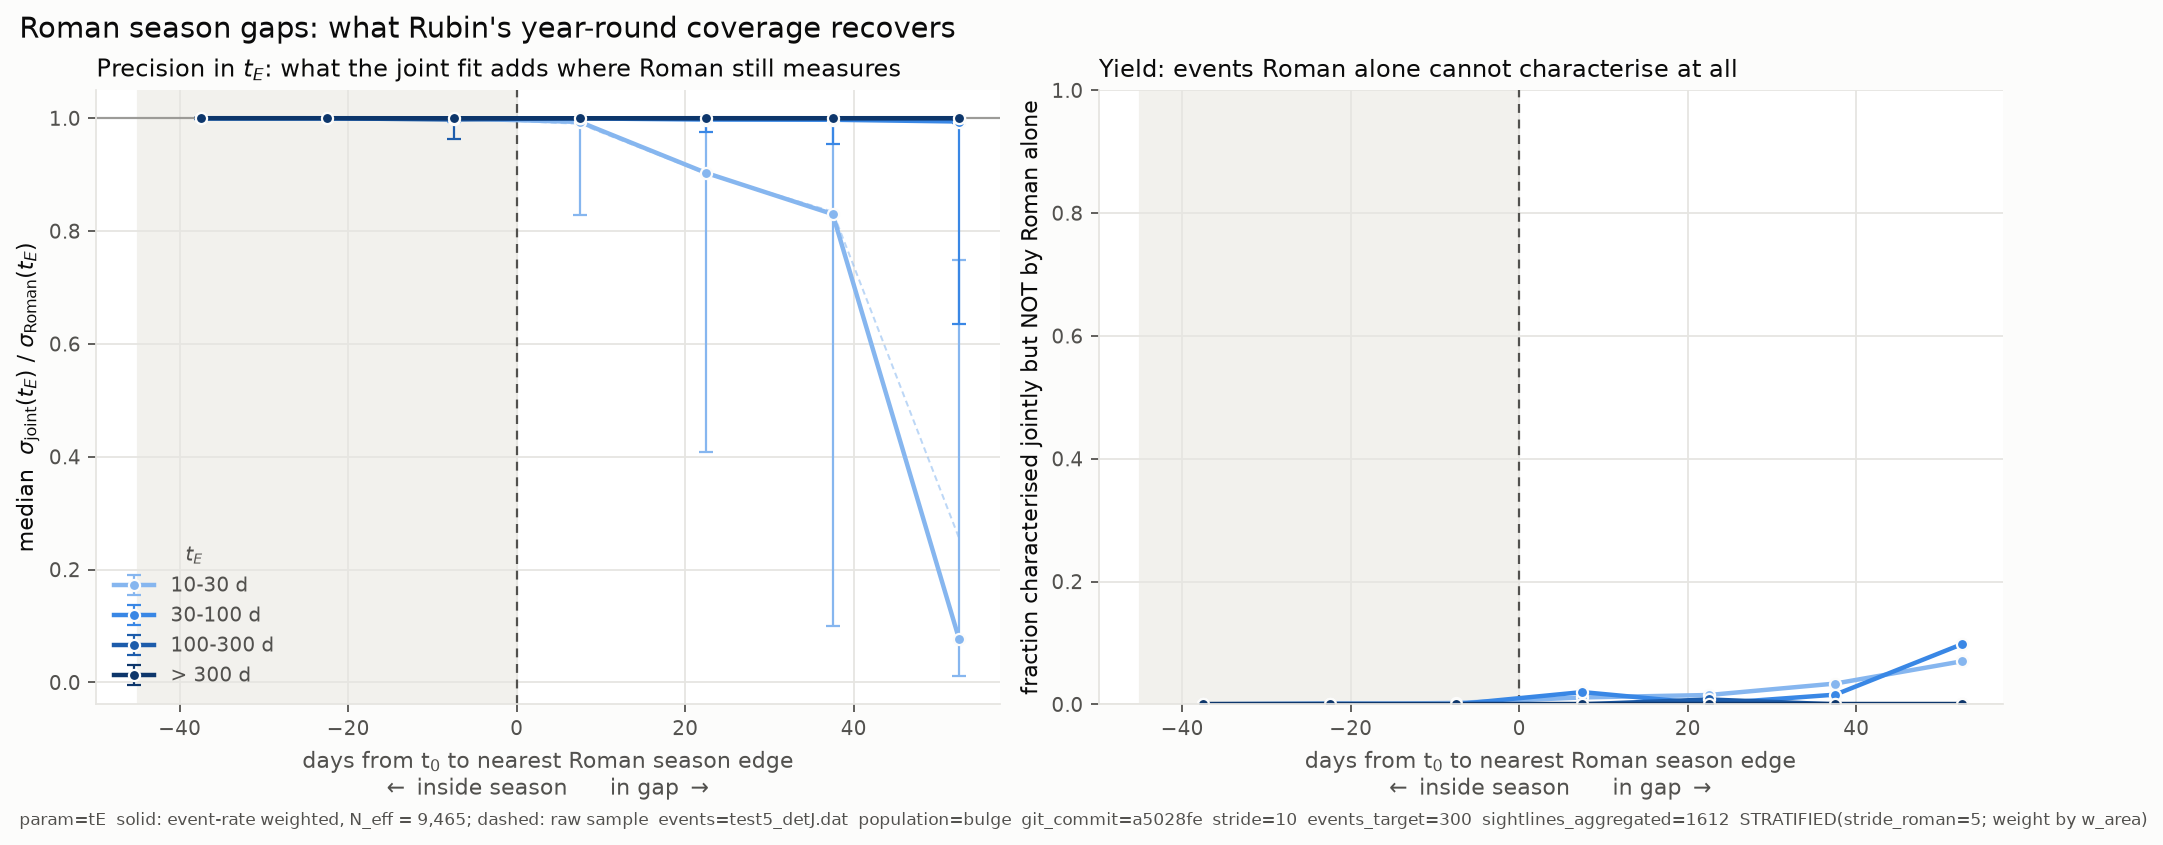
\includegraphics[width=\linewidth]{f2_gap_filling}
\refnote{Left: median $\sigma_{\rm joint}(\tE)/\sigma_{\rm Roman}(\tE)$ against the peak's distance from a season edge,
per $\tE$ bin. Right: fraction characterised jointly but not by Roman. Shaded: inside a season.}
\end{column}
\begin{column}{.42\linewidth}
\footnotesize
$10$--$30$\,d events, by where the peak falls:\\[2pt]
\begin{tabular}{@{}lcc@{}}
\toprule
peak & $\dfrac{\sigma_{\rm joint}}{\sigma_{\rm Roman}}(\tE)$ & $\Neff$ \\
\midrule
anywhere in a gap & $0.97$ & $670$ \\
$>15$\,d past an edge & $0.83$ & $376$ \\
$>30$\,d past & $0.44$ & $177$ \\
$>45$\,d past & $\mathbf{0.08}$ & $62$ \\
in a season & $1.00$ & $888$ \\
\bottomrule
\end{tabular}
\begin{itemize}
  \item Roman itself detects $96\%$ of in-gap events, from the wings
  \item The gain is largest for short events deep in a gap
  \item As simulated, without the later dust adjustment
\end{itemize}
\end{column}
\end{columns}
\end{frame}

\begin{frame}{Backup: two parallax baselines}
\begin{columns}[T]
\begin{column}{.52\linewidth}
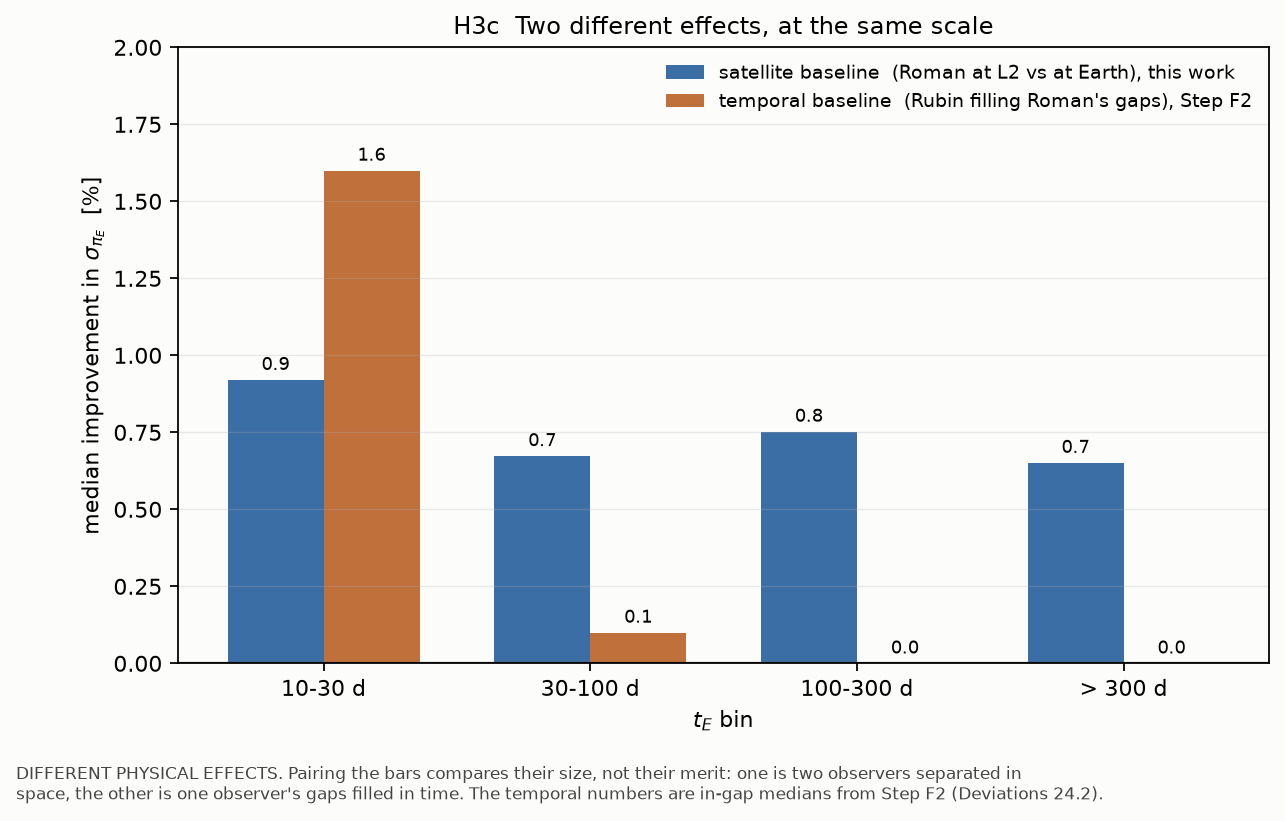
\includegraphics[width=\linewidth]{h3c_honest}
\refnote{Median improvement in $\sigma(\piE)$ per $\tE$ bin. Blue: Roman at L2 vs Roman at Earth (spatial).
Orange: joint vs Roman for events peaking in a gap (temporal).}
\end{column}
\begin{column}{.46\linewidth}
\small
\textbf{Spatial} (L2 vs Earth, $0.01$\,AU): each event forecast twice
\begin{itemize}\footnotesize
  \item Ordinary lenses: median error ratio $0.991$ ($\Neff=3{,}521$); $92\%$ improve
  \item $1.2\%$ improve by $>2\times$: short ($\tE\approx5$\,d), high-magnification events
  \item black holes and neutron stars: median ratio near one
\end{itemize}
\textbf{Temporal} (Rubin while Roman is not observing)
\begin{itemize}\footnotesize
  \item $10$--$30$\,d events: $1.6\%$ vs $0.9\%$ spatial
  \item large only for events wholly inside a gap
\end{itemize}
\end{column}
\end{columns}
\note{These ratios are conditional on the September orbit and noise models. The later orbit audit
      documented a bias in the legacy projection of Earth's orbit toward the bulge. The September
      median quantifies the paired test in that model. It is a historical forecast result.}
\end{frame}

\begin{frame}{Backup: what only the combination characterises}
\begin{columns}[T]
\begin{column}{.62\linewidth}
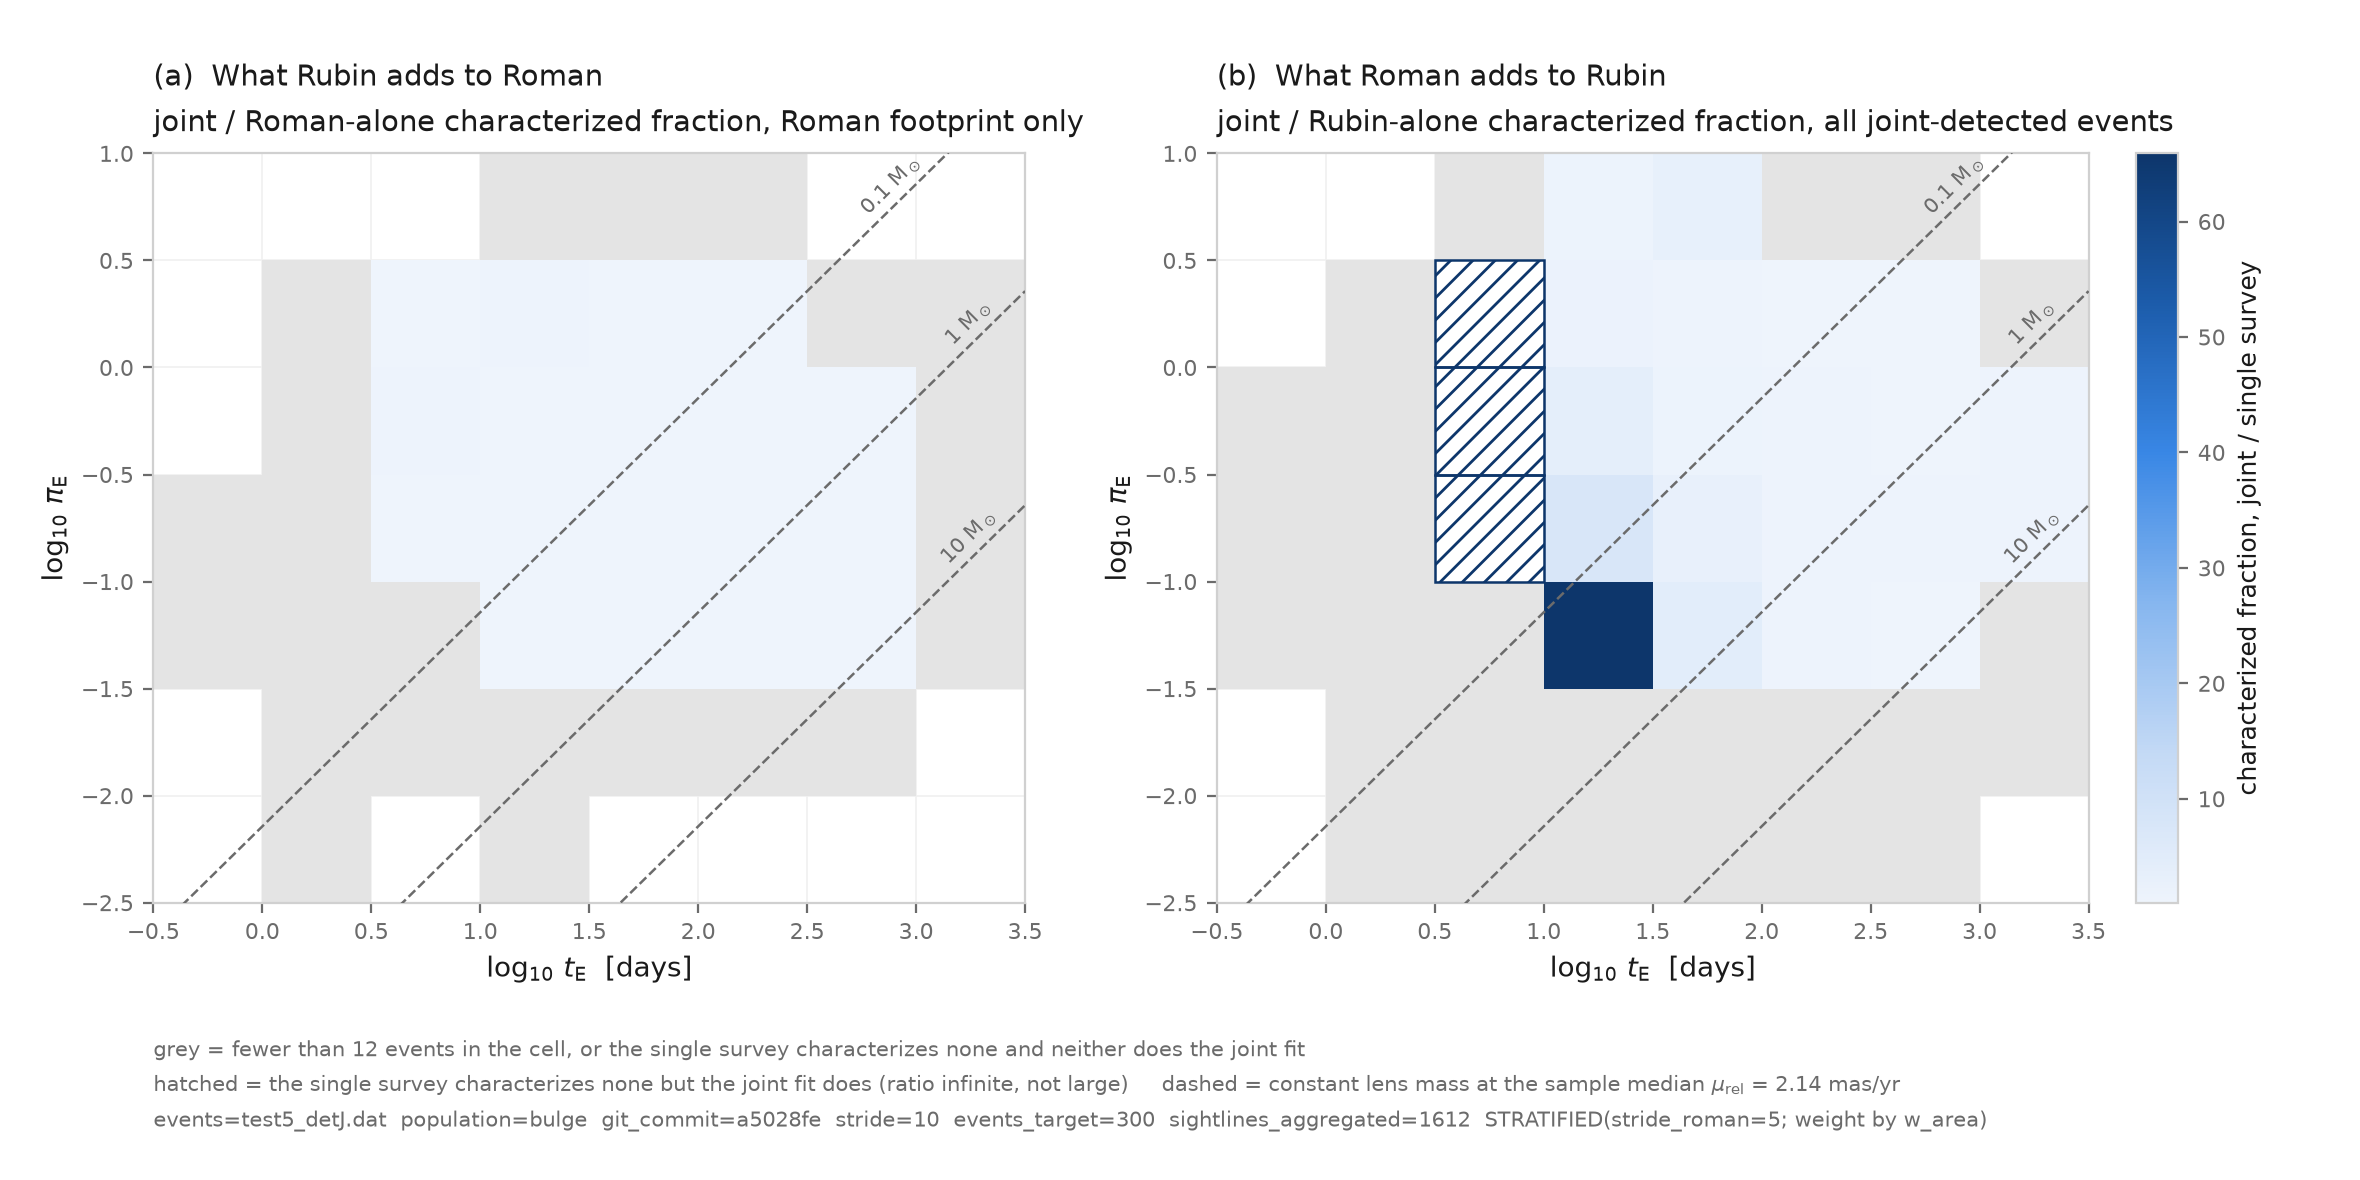
\includegraphics[width=\linewidth]{f3_characterization_map}
\refnote{Characterised fraction, joint over single survey, in the $(\tE,\piE)$ plane. (a) What Rubin adds to Roman;
(b) what Roman adds to Rubin (hatched: Rubin alone characterises none, the joint fit does). Dashed: constant mass.}
\end{column}
\begin{column}{.36\linewidth}
\small
\begin{itemize}
  \item (a) Adding Rubin changes the characterised sample little across most of this plane
  \item (b): Roman multiplies what Rubin can characterise, most for short events --- at $10$--$30$\,d and
        $\piE\sim0.03$--$0.1$, $66\times$
  \item $358$ of $12{,}461$ simulated footprint detections are characterised \emph{only} jointly: each survey holds part of the information
\end{itemize}
\end{column}
\end{columns}
\end{frame}

\begin{frame}{Backup: absolute precision, ordinary lenses}
\begin{columns}[T]
\begin{column}{.6\linewidth}
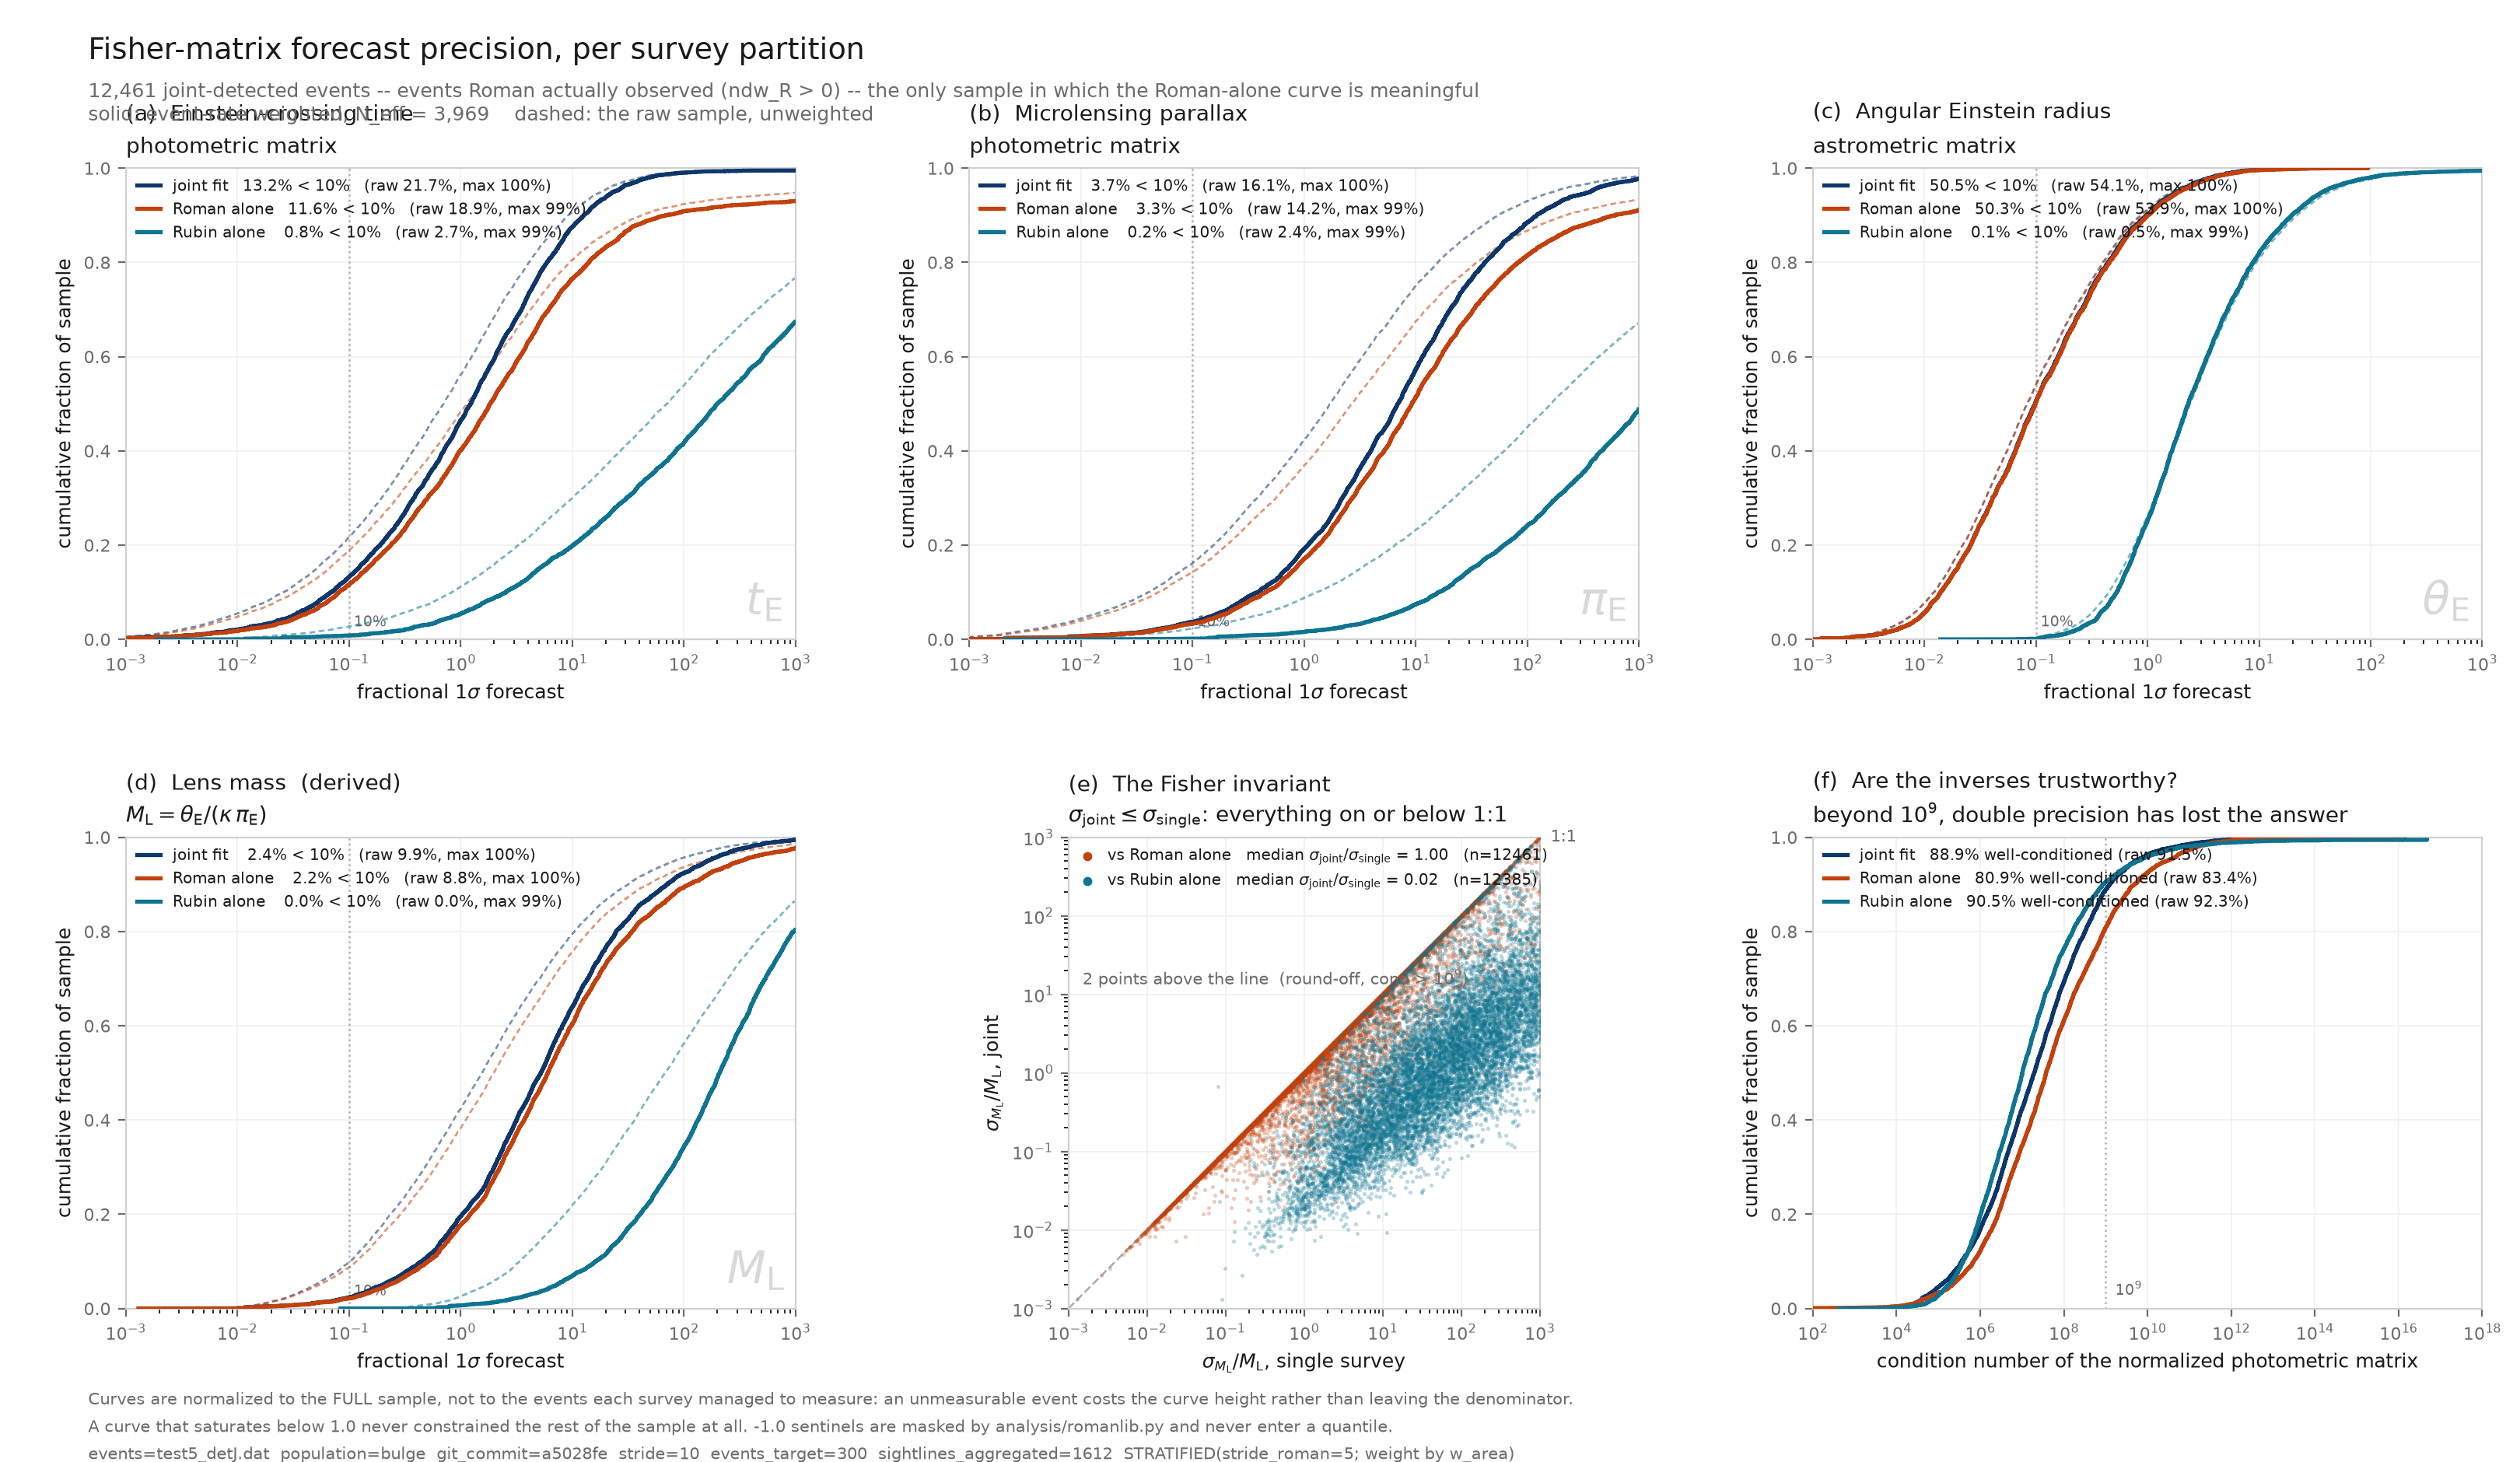
\includegraphics[width=\linewidth]{f4_fisher_precision}
\refnote{Fractional $1\sigma$ forecasts per survey over Roman's footprint detections ($\Neff\approx4{,}000$):
(a--c) fitted parameters, (d) mass, (e) $\sigma_{\rm joint}\le\sigma_{\rm single}$ event by event, (f) condition numbers.}
\end{column}
\begin{column}{.38\linewidth}
\small
Weighted \% measured to $10\%$ (as simulated):\\[3pt]
\begin{tabular}{@{}lccc@{}}
\toprule
 & joint & Roman & Rubin \\
\midrule
$\tE$ & $13.2$ & $11.6$ & $0.8$ \\
$\piE$ & $3.7$ & $3.3$ & $0.15$ \\
$\tetE$ & $50.5$ & $50.3$ & $0.13$ \\
$\Ml$ & $2.4$ & $2.2$ & $0.001$ \\
\bottomrule
\end{tabular}
\vspace{2mm}
\begin{itemize}\footnotesize
  \item the parallax is the limiting measurement
  \item unweighted the mass fraction is $9.9\%$: the raw sample over-represents long, slow events --- the weighting matters
\end{itemize}
\end{column}
\end{columns}
\end{frame}

\begin{frame}{Backup: compact objects in detail}
\centering
\small
\renewcommand{\arraystretch}{1.15}
\begin{tabular}{lrr}
\toprule
 & black holes & neutron stars \\
\midrule
detected by Rubin only / Roman only / both [\%] & $72.9$ / $21.5$ / $5.6$ & $69.6$ / $26.3$ / $3.9$ \\
median $\sigma_{\rm joint}/\sigma_{\rm Roman}$: $\tE$, $\piE$, $\tetE$ & $0.997$, $0.998$, $0.999$ & $0.999$, $0.999$, $0.999$ \\
median $\sigma_{\rm joint}/\sigma_{\rm Rubin}$: $\tE$, $\piE$, $\tetE$ & $0.022$, $0.010$, $0.041$ & $0.008$, $0.008$, $0.035$ \\
median maximum centroid shift & $3.60$\,mas & $0.26$\,mas \\
above Roman's $1.1$\,mas floor [\%] & $90.4$ & $0.6$ \\
Roman to $10\%$: $\tE$ / $\piE$ / $\tetE$ / $\Ml$ [\%] & $24$ / $13$ / $97$ / $13$ & $16$ / $4.5$ / $67$ / $3.7$ \\
\bottomrule
\end{tabular}

\vspace{4mm}
\begin{itemize}\small
  \item The $\sigma$ ratios use events with invertible photometric matrices for both surveys.
  \item The $10\%$ fractions use the available Roman forecasts ($\Neff\approx8{,}700$ for black holes,
        $\approx8{,}500$ for neutron stars).
\end{itemize}
\vfill
\refnote{As simulated. Detection and shift rows use all detections ($\Neff\approx17{,}000$ per population).}
\end{frame}

\begin{frame}{Backup: yields per unit abundance}
\centering
\small
Dust-adjusted ten-year yields per unit abundance inside the model footprint, except the final row.\\[4pt]
\renewcommand{\arraystretch}{1.15}
\begin{tabular}{lrrr}
\toprule
selection & black holes & neutron stars & ordinary ($F=1$) \\
\midrule
Roman detects & $5{,}660\pm320$ & $36{,}500\pm2{,}300$ & $50{,}400\pm2{,}900$ \\
Rubin detects & $690$ & $3{,}620$ & $4{,}850$ \\
both detect & $650$ & $2{,}220$ & $2{,}970$ \\
Rubin only & $23$ & $1{,}290$ & $1{,}820$ \\
\midrule
Roman, $\sigma_M/M<10\%$ & $579\pm42$ & $1{,}100\pm70$ & $830\pm110$ \\
joint, $\sigma_M/M<10\%$ & $650$ & $1{,}240$ & $900$ \\
Roman, $\sigma_M/M<1\%$ & $26$ & $20$ & $3$ \\
\midrule
Rubin detects, all $59$\,deg$^2$ & $11{,}200$ & $62{,}400$ & $78{,}300$ \\
\bottomrule
\end{tabular}

\vspace{3mm}
Multiply by $F$, the assumed stellar-mass share of the population. At fixed geometry and speed, higher mass increases each lens's cross-section but reduces the number of lenses per unit mass.
\end{frame}

\begin{frame}{Backup: the sky that was simulated}
\begin{columns}[T]
\begin{column}{.58\linewidth}
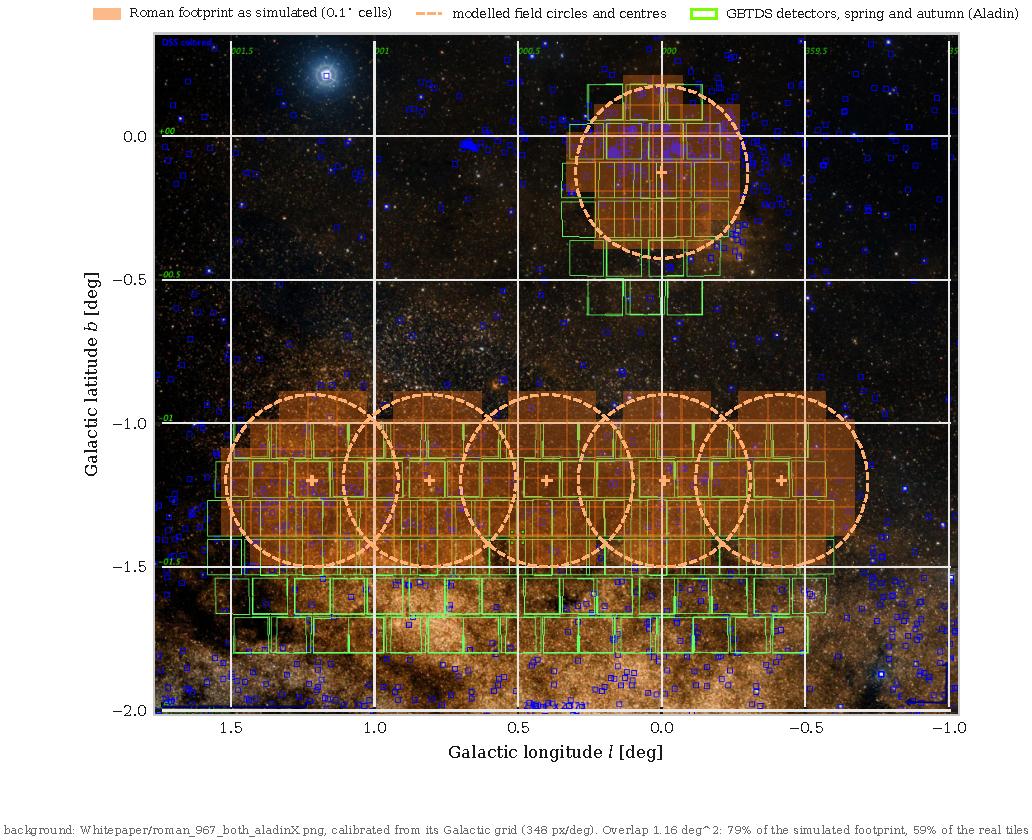
\includegraphics[width=\linewidth]{footprint_vs_gbtds}
\credit{background: \ads{2000A\%26AS..143...33B}{Aladin} (CDS), DSS images}
\end{column}
\begin{column}{.40\linewidth}
\small
\begin{itemize}
  \item $1{,}829$ sightlines over $68$\,deg$^2$: a Rubin exposure that contains part of a Roman field reaches $3.5^\circ$ beyond it
  \item $0.1^\circ$ grid inside Roman's fields ($147$ sightlines), $0.2^\circ$ outside; each carries its area
  \item Roman as simulated (orange): six circles, $1.47$\,deg$^2$, $\sim\!0.2^\circ$ closer to the plane than the adopted
        layout (green)
  \item The adopted detector geometry motivates a new footprint calculation
\end{itemize}
\end{column}
\end{columns}
\end{frame}

\begin{frame}{Backup: from the simulated sample to the sky}
\begin{itemize}
  \item The Monte Carlo does not draw events in proportion to the event rate: the lens mass and velocity draws miss a
        factor $\sqrt{\Ml}\,v_t$
  \item Each event therefore carries a weight $W\propto$ its event rate; every pooled fraction or median is weighted
  \item The weight costs precision; it is quoted as the Kish effective sample size
  \[
    \Neff = \frac{\left(\sum W\right)^2}{\sum W^2}
  \]
        e.g.\ $12{,}461$ simulated footprint detections weigh as $\Neff\approx4{,}000$
  \item Populations are never pooled: the weight contains $\sqrt{M}$ of the population drawn
  \item Yields: the weighted sample normalised to an expected number of events, $N(F)=F\,N_1$
  \item \textbf{Check:} mean event timescale in the comparison sightlines is $23.5$\,d, versus $23.8$\,d from OGLE-IV
\end{itemize}
\vfill
\refnote{\ads{2019ApJS..244...29M}{Mr\'oz et al.\ 2019, ApJS 244, 29}}
\end{frame}

\begin{frame}{Backup: the dust near the Galactic plane}
\begin{itemize}
  \item A declination rule assigned almost all model Roman sightlines to Bayestar. Within
        $\sim\!1^\circ$ of the plane it gives \textbf{3--6 times too little} extinction, measured against the VVV
        reddening map
  \item After reweighting outcomes against dust checked with VVV:
  \begin{itemize}
    \item Roman's yields $-33$ to $-38\%$ (its $10\%$ masses $-46$ to $-57\%$); Rubin's $-54$ to $-71\%$
    \item Roman retains the stronger precision within its footprint
    \item Roman's detection rate becomes $(23\pm5)\%$ below Penny et al.\ for the same $u_0$ range
  \end{itemize}
  \item \textbf{Dust-model update.} Rebuild the extinction tables from DECaPS, with near-infrared dust where DECaPS saturates;
        check against VVV before any run
\end{itemize}
\vfill
\refnote{\ads{2019ApJ...887...93G}{Green et al.\ 2019};
\ads{2025ApJ...992...39Z}{Zucker et al.\ 2025};
\ads{2020A\%26A...644A.140S}{Surot et al.\ 2020};
\ads{2006A\%26A...453..635M}{Marshall et al.\ 2006};
\ads{2019ApJS..241....3P}{Penny et al.\ 2019}}
\end{frame}

\begin{frame}{Backup: comparison with Sajadian \& Sahu (2023)}
This simulation builds on the paper's approach (separate photometric and astrometric Fisher matrices). With its mass
function ($dN/dM\propto M^{-1}$) and on its sample ($u_0<1$, peak inside the mission):
\vspace{2mm}
\begin{center}
\renewcommand{\arraystretch}{1.15}
\begin{tabular}{lcccc}
\toprule
\% to $10\%$ & $\tE$ & $\piE$ & $\tetE$ & $\Ml$ \\
\midrule
Sajadian \& Sahu 2023 & $67.0$ & $30.0$ & $99.2$ & $29.8$ \\
this work, rate-weighted & $67.4$ & $23.5$ & $75.5$ & $21.1$ \\
this work, per simulated event & $71.9$ & $42.1$ & $80.2$ & $38.1$ \\
\bottomrule
\end{tabular}
\end{center}
\begin{itemize}\small
  \item The weighted $\tE$ share is close. The published $\piE$ and mass shares lie between the two counting conventions shown here.
  \item $\tetE$ differs. The analyses use different astrometric noise models and treat parallax differently in the centroid fit.
\end{itemize}
\vfill
\refnote{\ads{2023AJ....165...96S}{Sajadian \& Sahu 2023}. The weighted comparison has $\Neff=1{,}472$. Detection cuts also differ.}
\end{frame}

\begin{frame}{Backup: a distant black hole}
\begin{columns}[T]
\begin{column}{.66\linewidth}
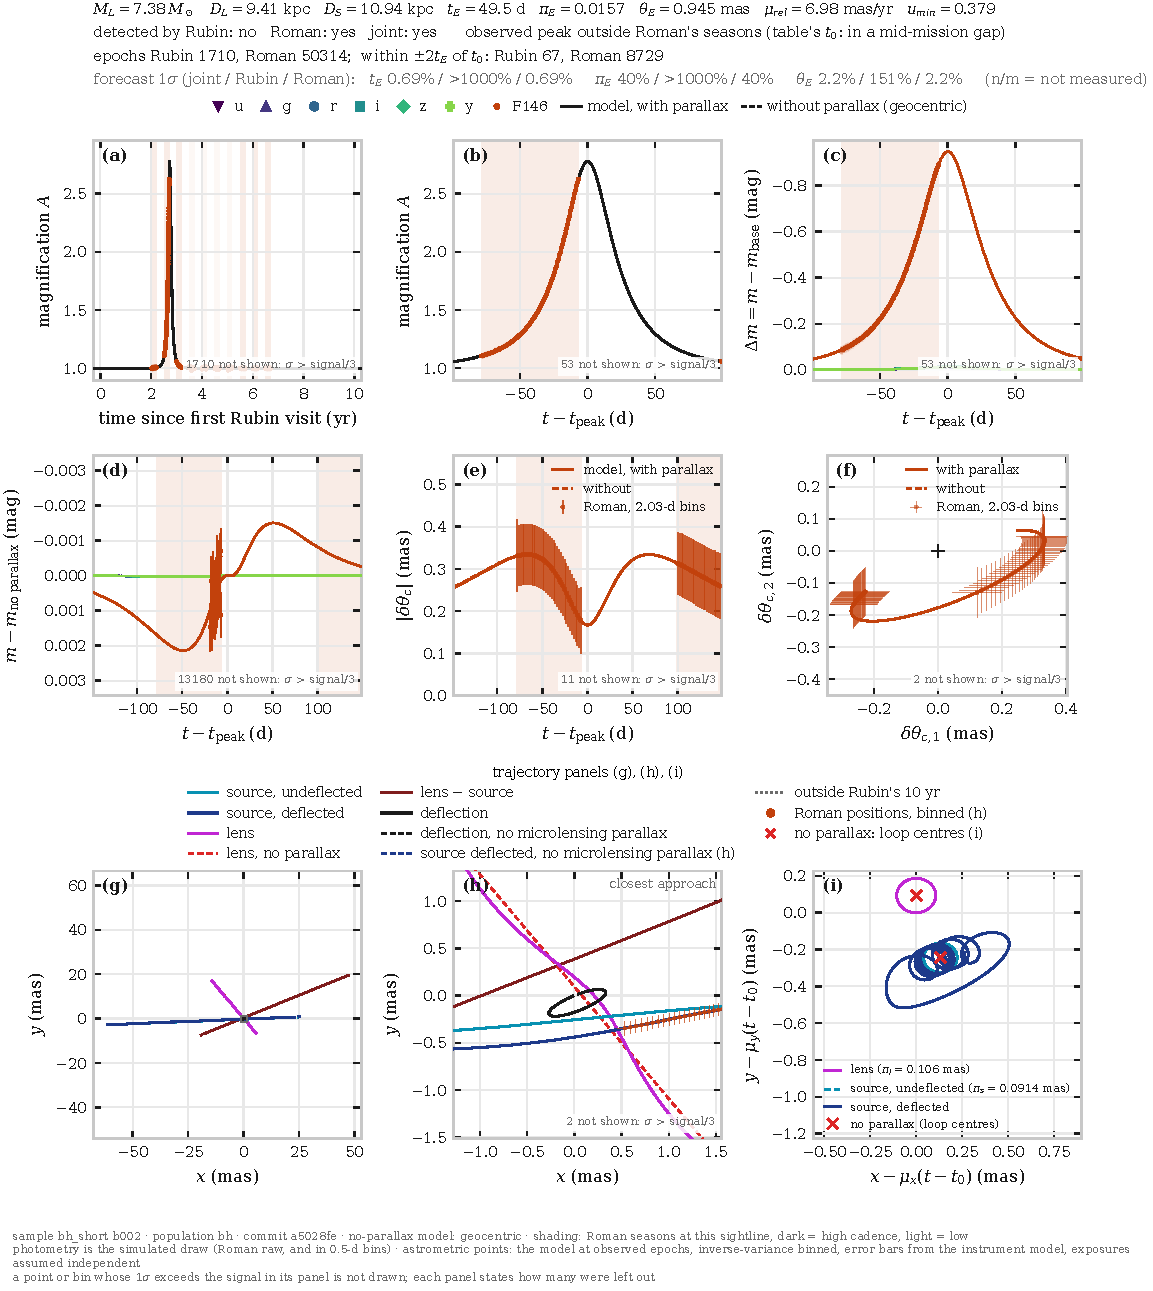
\includegraphics[width=\linewidth, trim=0 255 0 0, clip]{bh_short_b002_3x3}
\end{column}
\begin{column}{.32\linewidth}
\small
\textbf{$7.4\,\Msun$ at $9.4$\,kpc}, behind the Galactic centre; $\tE=50$\,d
\begin{itemize}
  \item Roman alone: $\tE$ to $0.7\%$, $\tetE$ to $2.2\%$
  \item but $\piE$ is tiny: \textbf{mass only to $\sim\!40\%$}
  \item Rubin does not detect it
\end{itemize}
The parallax limit in one event.
\end{column}
\end{columns}
\vfill
\refnote{September sample gallery, event bh\_short\_b002.}
\end{frame}

\begin{frame}{Backup: resolving the images --- the criterion}
\begin{itemize}
  \item At every visit: (i) both images detectable on their own (between saturation and the single-visit depth; blended
        light not added back); (ii) $\Delta\theta=\tetE\sqrt{u^2+4}$ above a bar
  \item Resolvable: $\ge3$ such visits
  \item Bars: $\mathcal{D}\sigma_{\rm ast}$ with $\mathcal{D}\approx5$ (detection limit) to $\approx20$ (S/N $\sim100$),
        built for Rubin's seeing-limited images; the PSF width ($105$\,mas for Roman, $\approx1''$ for Rubin)
  \item On Roman's $1.1$\,mas floor, $\mathcal{D}=5$ means separating sources $5.5$\,mas apart --- a twentieth of its PSF
  \item Roman's depth taken as F146 $=25.5$ ($5\sigma$, single exposure)
\end{itemize}
\vspace{2mm}
\centering\small
\begin{tabular}{lccc}
\toprule
Roman (dust-corrected) [\%] & black holes & neutron stars & ordinary \\
\midrule
$\mathcal{D}=5$ & $34$ & $1.7$ & $0.8$ \\
$\mathcal{D}=20$ & $15$ & $0.02$ & $\approx0$ \\
PSF & $0.25$ & $\approx0$ & $0$ \\
\bottomrule
\end{tabular}
\vfill
\refnote{\ads{2026ApJ..1009..116S}{Sajadian \& Makler 2026, ApJ 1009, 116}}
\end{frame}

\begin{frame}{Backup: how sensitive are the first results?}
\centering
\footnotesize
\renewcommand{\arraystretch}{1.12}
\begin{tabular}{p{.50\linewidth}p{.12\linewidth}p{.28\linewidth}}
\toprule
result & confidence & main risk \\
\midrule
For shared events, median timescale gain from Rubin is $<0.4\%$ & high & Roman photometric noise \\
Roman turns Rubin's detections into measurements & high & noise; astrometric floor \\
$\sim\!60\%$ of ordinary-lens detections are outside Roman's fields & high & latitude gradient \\
gap filling: only deep in gaps, short events & medium & small $\Neff$; not dust-corrected \\
negligible median satellite-parallax gain for black holes & high & September orbit model \\
black-hole $\tetE$ & high & --- \\
ordinary and neutron-star $\tetE$ and masses & medium--low & correlated astrometric floor \\
absolute yields $N_1$ & medium--low & dust near the plane \\
yields $N(F)$ & low & $F$ unknown to $\times6$ \\
image resolution & low & the criterion for Roman \\
\bottomrule
\end{tabular}
\end{frame}

\begin{frame}{Backup: Roman's adopted field layout}
\centering
\vspace{2mm}
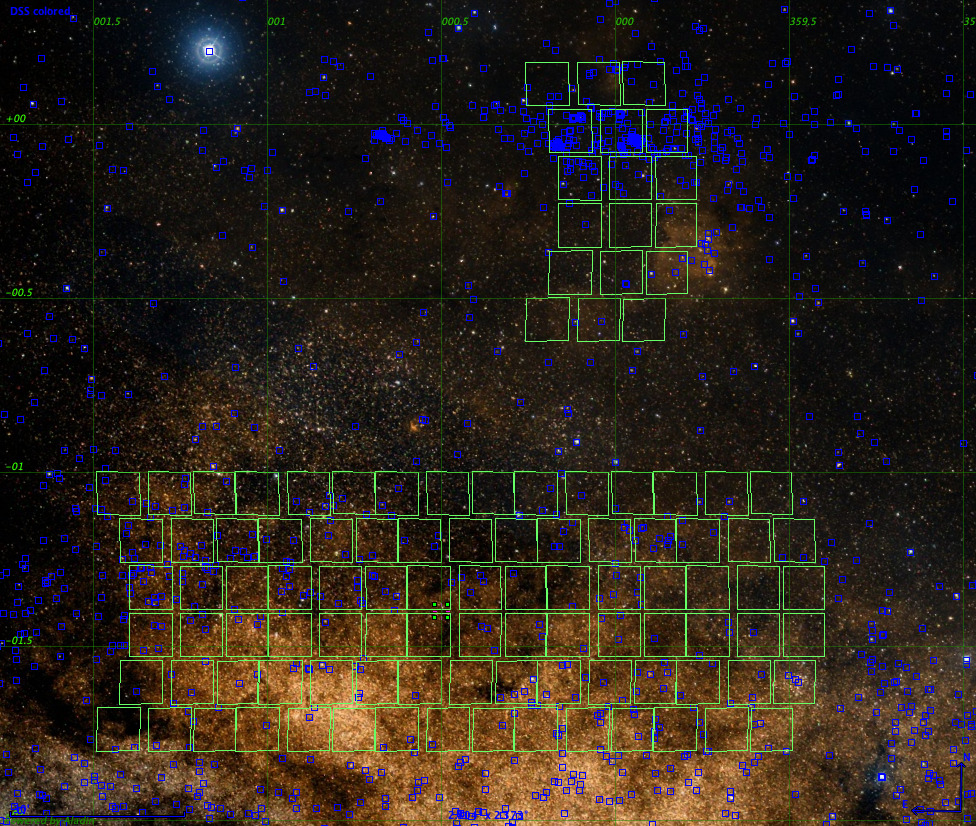
\includegraphics[width=.42\linewidth]{roman_gbtds_fields_spring}\hspace{6mm}%
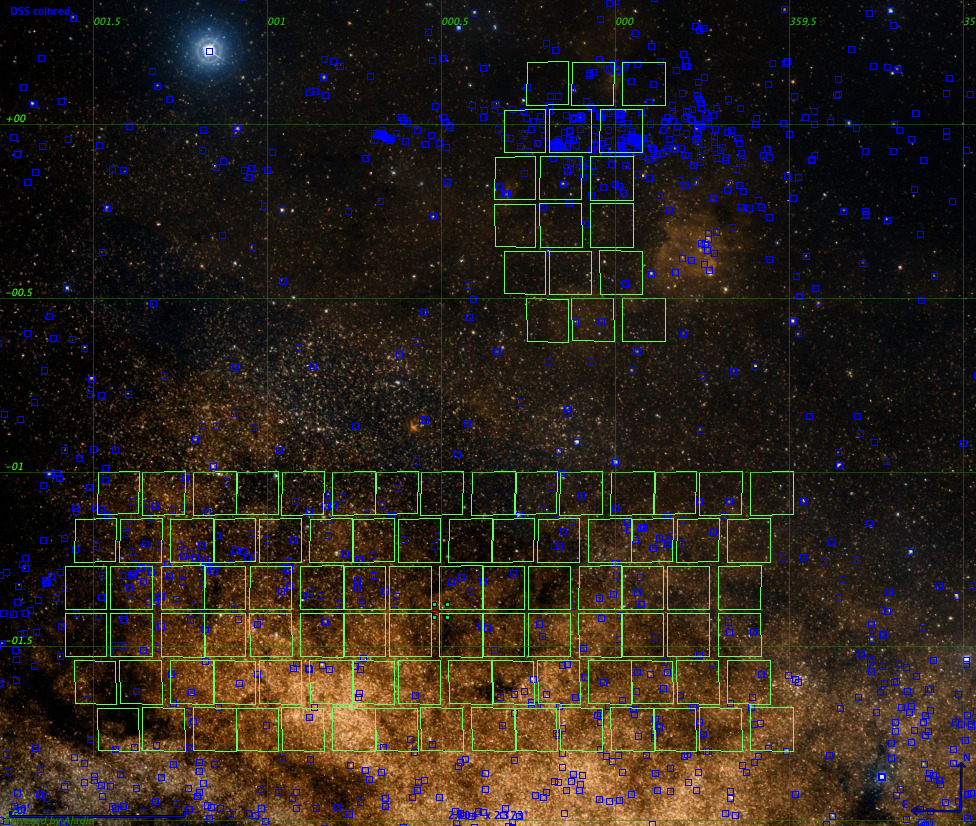
\includegraphics[width=.42\linewidth]{roman_gbtds_fields_autumn}\\[1mm]
\credit{\href{https://roman-docs.stsci.edu/roman-community-defined-surveys/galactic-bulge-time-domain-survey}{STScI, Roman GBTDS}}\\[2pt]
\small WFI detectors in the six GBTDS fields, spring (left) and autumn (right) seasons; the roll angle differs between them.
\end{frame}

\begin{frame}{Backup: forecasts in the literature}
\begin{columns}[T]
\begin{column}{.48\linewidth}
\centering
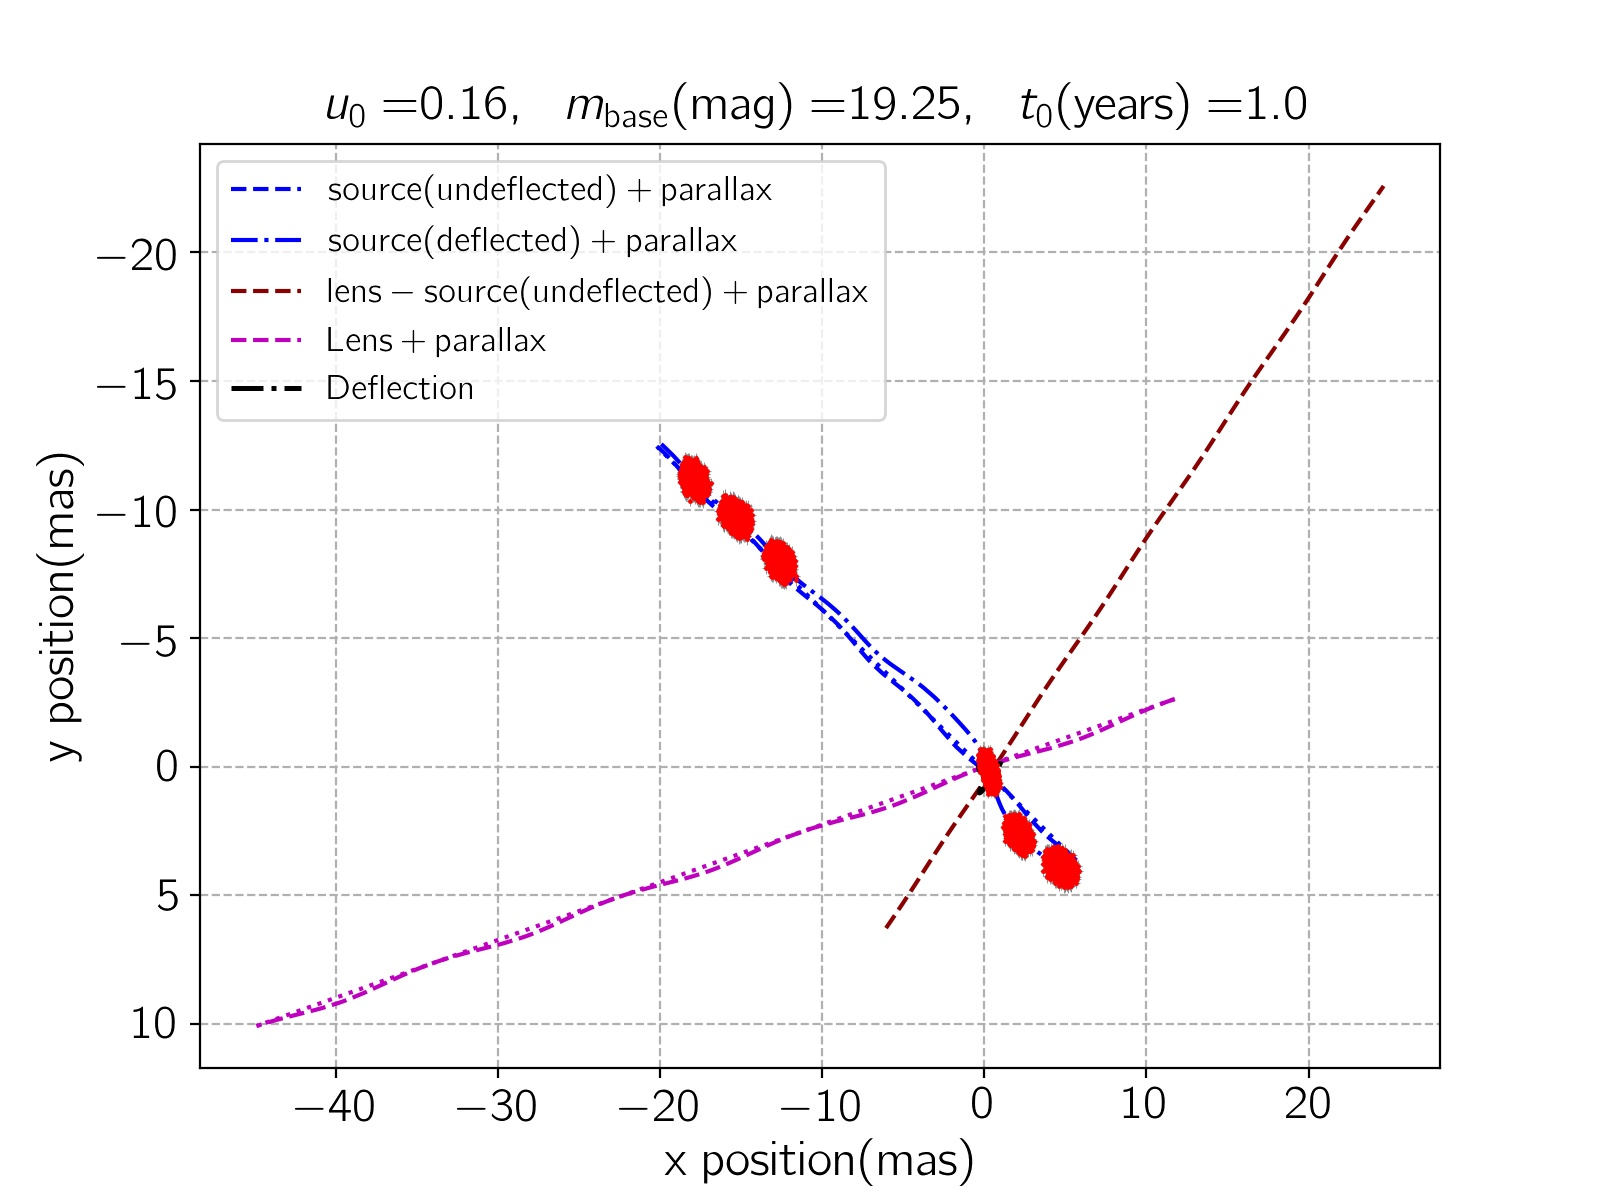
\includegraphics[width=.9\linewidth]{ss23_astrometry}
\credit{\ads{2023AJ....165...96S}{Sajadian \& Sahu 2023, AJ 165, 96}}\\
\footnotesize Roman: a simulated black-hole event, the source and lens tracks on the sky with the astrometric deflection.
\end{column}
\begin{column}{.48\linewidth}
\centering
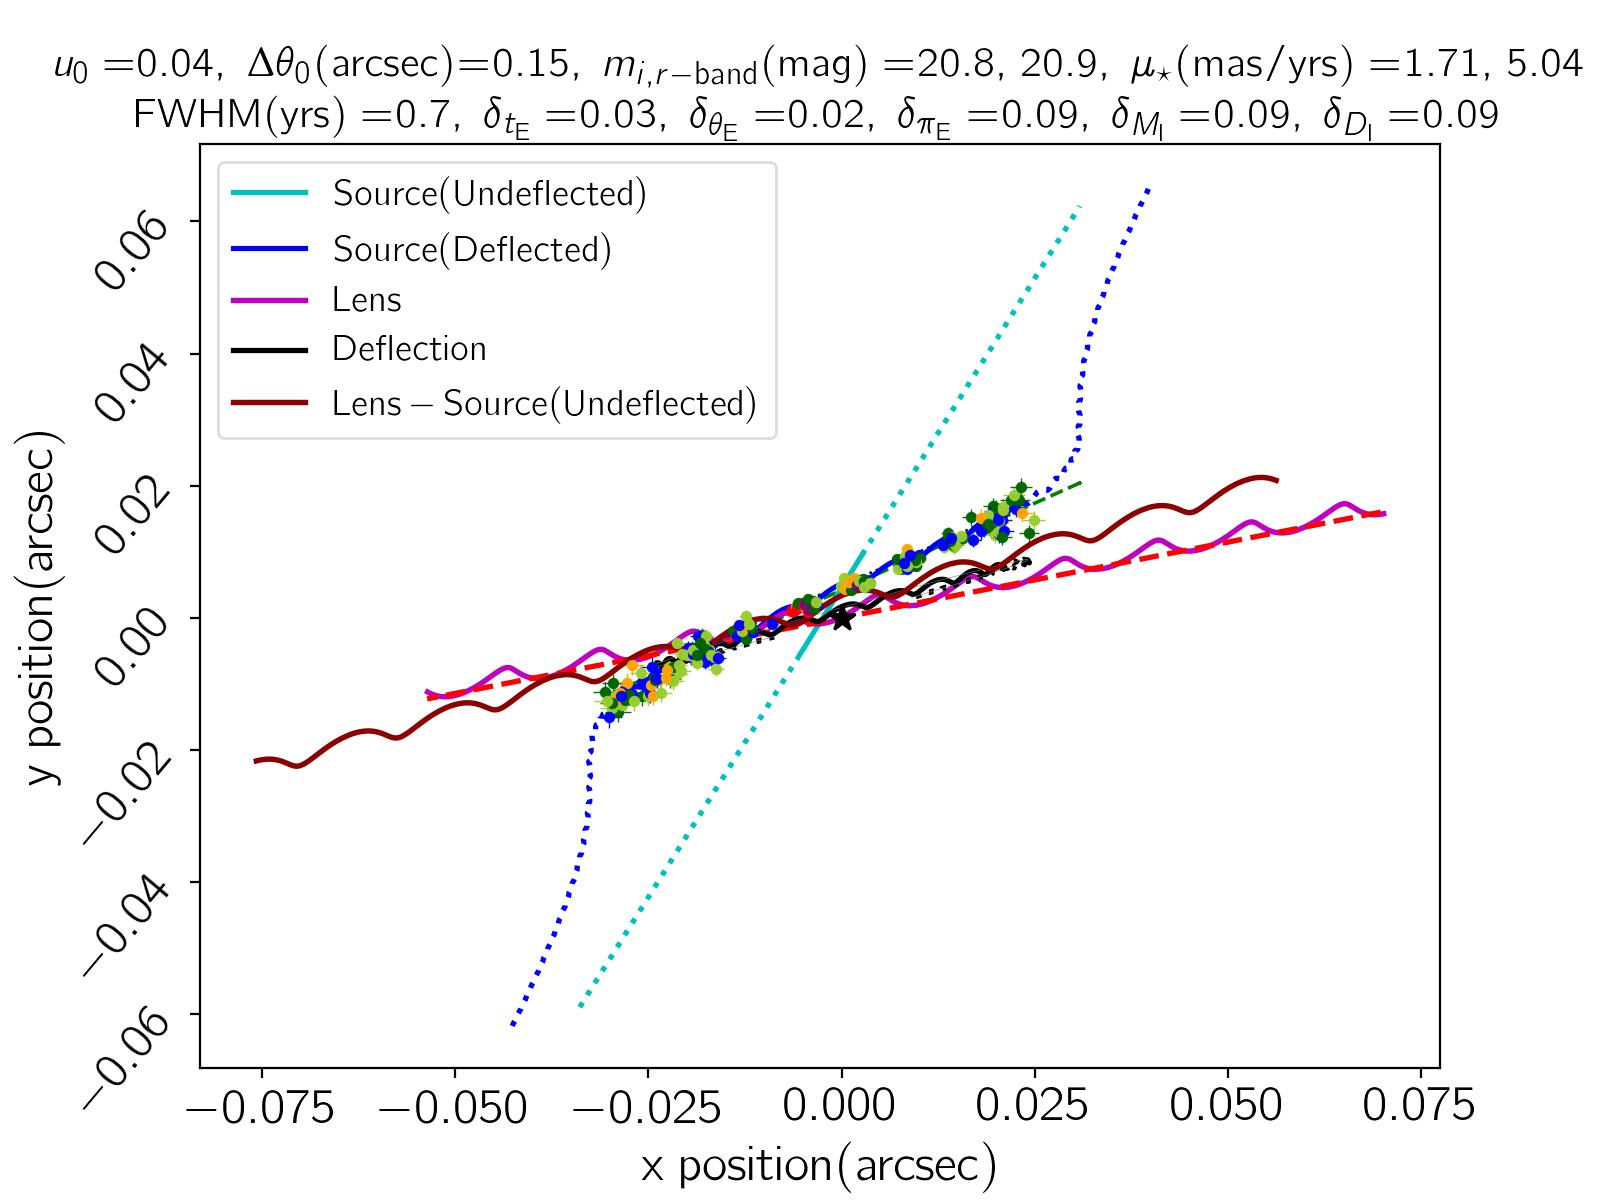
\includegraphics[width=.9\linewidth]{sm26_astrometry}
\credit{\ads{2026ApJ..1009..116S}{Sajadian \& Makler 2026, ApJ 1009, 116}}\\
\footnotesize Rubin toward the Large Magellanic Cloud: a $422\,\Msun$ simulated lens at $0.6$\,kpc, $\tE=5.4$\,yr, $\tetE=73$\,mas.
\end{column}
\end{columns}
\end{frame}
